\section{Biological Nanopores}

Biological nanopores are small perforations in the bi lipid membrane, created by a pore
forming protein.  These proteins are toxins
produced by bacteria, as means of killing targeted cells. They work by perforating
the cell membrane of a cell, of which the contents is spilled into the
environment though osmoses, thereby killing the cell.

The small scale of these protein structures, a few nanometers across,


due to their small scale ideal for spectroscopy.

short introduction to their structural.

should be noted that also solid state nano pores exist poking hole in semi conductor.
Prescission is much less so currently bio pores are better. Interesting future.


\subsection{$\alpha$-Hemolysin ($\alpha$ HL)}


- beta nano pore
- secreted by Staphylococcus aureus in its post-exponential and stationary growth phases
- sevon subunits of monomers ->  mushroom shape protein complex, h11nm by w10nm.
- small diamater -> single stranded DNA passes through.
- neutral charge, important for translocation of charged analytes.
- monomers bind to cell membrane, collide to form 'prepore'
- the stem is inserted into the membrane to from the nano pore
-


\begin{figure}[h!]
  \centering
  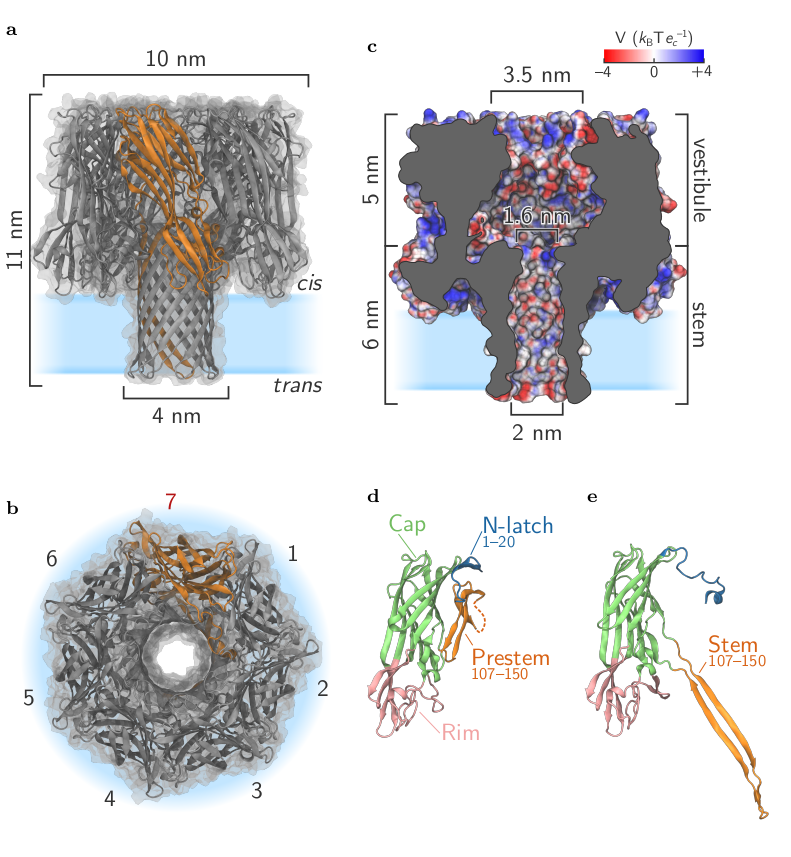
\includegraphics[width=0.5\linewidth]{Figures/alpha-hemolysin.png}
  \caption{write caption}
  \label{adsf}
\end{figure}


\subsection{Cytolysin A (ClyA)}

- alpha nano pore
- secreted by various S. enterica and E. coli strains
- 12,13,14 subunits of monomers ->  mushroom shape protein complex, h14nm by w11nm.
- all have different constriction widths
The interior shape of ClyA can be described
as a set of two hollow cylinders placed on top of each other: a large cis chamber
(‘lumen’) with an inner diameter of ≈5.5 nm and a height of 10 nm and a smaller
trans chamber (‘constriction’) with a width of ≈3.6 nm and a height of 4 nm

- large diamater -> study large bio molecules, double stranded DNA passes through
important for futher in thesis.

- negaive charge in interior of pore, important for translocation of charged analytes.
- monomers bind to cell membrane  due to hydrophobic parts of monomers.
- next alpha helix hairpin hinges and connects to membrane, forming the nano pore.
similar to that of a spring-loaded lock, which is opened upon membrane binding


\begin{figure}[h!]
  \centering
  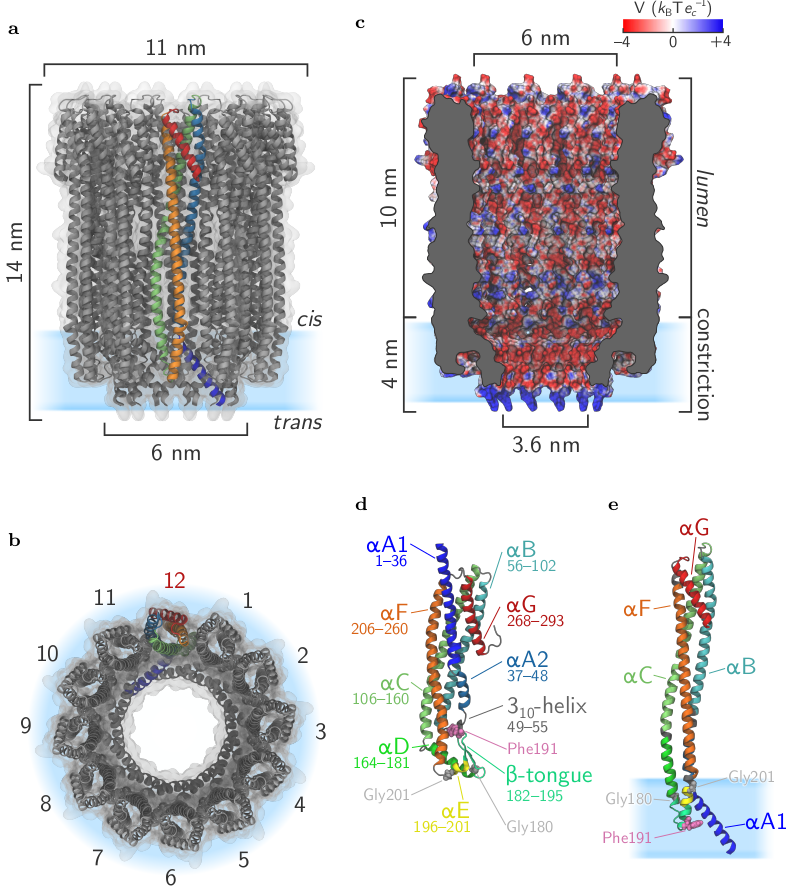
\includegraphics[width=0.5\linewidth]{Figures/cytolysinA.png}
  \caption{write caption}
  \label{adassf}
\end{figure}

\subsection{Ionic current spectroscopy}
In recent years the study nanopores became a popular research domain, mainly
due to the development of the nanopore-based ionic current spectroscopy. for the case of
biological nanopores, this method depicted in figure .., a bilipid membrane is perforated
using a pore froming protein like $\alpha$- HL. The membrane seperates two chambers of
basin filled with a saline solution. The created nanopore acts a the sole connection
between the two sides of this basin. Next a potential diffrence is created over the
membrane, which induces a ion current through the nanopore.

This field induces several distinct forces that influence
the movement of analyte molecules towards and within the pore (Fig. 1.10):
the electrophoretic (EP), electro-osmotic (EO) and dielectrophoretic (DEP)
forces. The former two are the strongest, and hence also the most well-known.
Besides attracting analytes and inducing their translocation, external forces may
also impact the structure of the molecules themselves

- open pore current
- characterasing blocked currents -> single cell spectroscopy.

It should be noted that besides these biological nanopores, there are also solid state
nanopore under development. While they are currently not as accurate as biological
nanopres, mainly due to their size difference, this method would allow for more
specialised modelling of these nanopores. often times solid state nanopores are created
by perforating a semi conductor wafer, changing the diameter and shape of this
perforation would allow for  case specific nanopore development. While thus currently not
as widely used as biological nanopores, due to this customisability solid state nanopores
are the future of nanopore technology.
